\section{Mutual Exclusion} \label{sec:mutex}

Data races in parallel programs lead to non-deterministic behavior of programs. Therefore, data races are termed as errors. When access to a shared variable is protected by a lock, there is a programmer intended race on the variable. When these accesses are not ordered by the programmer, the output of the program is becomes non-deterministic. This behavior, however, is expected by the programmer. 

Programs with data races can have different computation graph structures based on the schedule of tasks in the runtime (i.e., different update orders may result in different control flow paths). Similarly, when shared memory accesses are protected using locks, different computation graph structures can be observed based on the order in which the tasks access the protected shared variable. To ensure that a program in which tasks have mutually exclusive access to some shared variable does not have any unintended race, all the computation graph structures that can result from different schedules over the protected shared variable access have to be enumerated and analyzed.

\begin{figure}[h]
\vspace{-1em}
  \begin{center}
\[
  \begin{array}{rcl}
\textbf{s} &::=& \textbf{isolated}~\texttt{l}\ := p~e~\vec{r_\delta}~\vec{r_\omega}
  \end{array}
\]
  \end{center}
  \caption{The surface syntax for task parallel programs extended with isolated}
  \label{fig:syntax-iso}
\end{figure}

The surface syntax of task parallel languages has been extended to include isolated statements as shown in \figref{fig:syntax-iso}. 
The \textbf{isolated} statement runs procedure $p$ in mutual exclusion with any other \textbf{isolated} procedure.

\begin{figure*}
  \begin{center}
    \mprset{flushleft}
    \begin{mathpar}
     \inferrule[Isolated]
     {
     }
     { 
     C[T[\textbf{isolated}~\texttt{l}\ := p~e~\vec{r_\delta}~\vec{r_\omega}], m] \rightarrow
      C[T[\textbf{isolated-post}~r_\mathit{is}\leftarrow p~e~\varepsilon~\vec{r_\delta}~\vec{r_\omega}~\lambda v.\texttt{l} := v;~\textbf{isolated-ewait}~r_\mathit{is}], m]
     }
      \and
      \inferrule[Isolated-Post]
                {
					\mathit{canIsolate()} = true \\
                  n_1 = \mathrm{fresh}() \\
                  N = N \cup \{n_1\} \\
                  E = E \cup \{\tuple{n, n_1},  \tuple{PrevIN,n_1}\}\\\\
                 PrevIN = n_1 \\
                  \ell \in e(\ell^\prime,\vec{r_\delta}^\prime) \\
                  \delta = \delta \cup (n \mapsto \eta(e))\\
                  m^\prime = (m \setminus m |_{\vec{r}}) \cup
                  (r \mapsto \tuple{
                    \tuple{\ell, s_p, d, \vec{r_\delta}, \vec{r_\omega},n_1},m|_{\vec{r}}})
                }
                {
                  C[\tuple{\ell^\prime, 
                  S[\textbf{isolated-post}~r \leftarrow p~e~\vec{r_\delta}~\vec{r_\omega}~d],\vec{r_\delta}^\prime,\vec{r_\omega}^\prime,d^\prime, n, false}, m] \rightarrow
                  C[\tuple{\ell^\prime,
				   S[\textbf{skip}],\vec{r_\delta}^\prime,\vec{r_\omega}^\prime,d^\prime, n, true}, m^\prime]
                }
      \and
            \inferrule[Isolated-Post-Nested]
                {
					\mathit{canIsolate()} = false~\&~iso = true\\
                  n_1 = \mathrm{fresh}() \\
                  N = N \cup \{n_1\} \\
                  E = E \cup \{\tuple{n, n_1},  \tuple{PrevIN,n_1}\}\\\\
                 PrevIN = n_1\\
                  \ell \in e(\ell^\prime,\vec{r_\delta}^\prime) \\
                  \delta = \delta \cup (n \mapsto \eta(e))\\
                  m^\prime = (m \setminus m |_{\vec{r}}) \cup
                  (r \mapsto \tuple{
                    \tuple{\ell, s_p, d, \vec{r_\delta}, \vec{r_\omega},n_1},m|_{\vec{r}}})
                }
                {
                  C[\tuple{\ell^\prime, 
                  S[\textbf{isolated-post}~r \leftarrow p~e~\vec{r_\delta}~\vec{r_\omega}~d],\vec{r_\delta}^\prime,\vec{r_\omega}^\prime,d^\prime, n, false}, m] \rightarrow
                  C[\tuple{\ell^\prime,
				   S[\textbf{skip}],\vec{r_\delta}^\prime,\vec{r_\omega}^\prime,d^\prime, n, true}, m^\prime]
                }
      \and
      \inferrule[Isolated-Ewait]
                {
                  n^\prime = \mathrm{fresh}() \\
                  N= N \cup \{n^\prime\} \\
                  E = E \cup \{\tuple{n, n^\prime}, \tuple{n(t_2),n^\prime}\} \\
                  m_1 = (r \mapsto \tuple{t_2,m_2}) \cup m_1^\prime \\
                  s \in \mathrm{rvh}(t_2)
                }
                {
                  C[\tuple{\ell,
S[\textbf{isolated-ewait}~r],\vec{r_\delta},\vec{r_\omega},d, n, true}, m_1] \rightarrow
                  C[\tuple{\ell,
S[s],\vec{r_\delta},\vec{r_\omega},d, n^\prime, false}, m_1' \cup m_2]
          }
\end{mathpar}
  \end{center}
  \caption{The transition rules for the isolated statements.}
  \label{fig:isol-semantics}
\end{figure*}

\figref{fig:isol-semantics} gives the semantics for \textbf{isolated} statement. The configuration is extended to include a boolean variable $iso$ that indicates the task is isolated. The \textbf{isolated-post} and \textbf{isolated-ewait} statements have also been added to the semantics. An \textbf{isolated} statement is interpreted as an \textbf{isolated-post} followed by an \textbf{isolated-ewait} statement on some region $r_{is}$. This region is exclusive to the isolated statement. No other tasks can post into this region.

The isolated-post statement fires either \textsc{Isolated-post} or \textsc{Isolated-post-nested} depending on the state of the system. The $\mathrm{canIsolate}$ method returns true if the boolean variable $iso$ is false for all the tasks in the program. If $\mathrm{canIsolate}$ returns true, \textsc{Ioslated-post} rule is fired. When $\mathrm{canIsolate}$ returns false, if the task executing \textbf{isolated} statement has $iso$ set to true, the \textsc{Isolated-post-nested} rule fires. If $iso$ is true for some other task, the execution of the \textbf{isolated-post} is blocked until $\mathrm{canIsolate}$ returns true.

The rules \textsc{Isolated-post} and \textsc{Isolated-post-nested} create a new node $n_1$ that represents the statements executed by the isolated procedure. The current node $n$ of task $t$ is connected to this new node $n_1$. If some other task has previously executed an isolated statement, a serialization edge is added from the isolated node of that task $PrevIN$ to $n_1$. The pointer $PrevIN$ is changed to point to the newly created node $n_1$ and the boolean identifier marking the execution of isolated is set to true.

When \textsc{Isolated-ewait} fires, a new node $n_1$ is created to represent the statements following the \textbf{isolated} statement. The current node $n$ of task $t$ is connected to this new node $n_1$. The current node of the task executing isolated procedure is also connected to node $n^\prime$. The boolean identifier marking the execution of isolated is set to false.

On-the-fly data race detection is modified for programs with isolated regions. When \textsc{Await-done} fires, the runtime checks if the region contains any task containing \textbf{isolated} statements. If the region does not have any isolated-nodes, data race detection is run on the region and if the region is data race free, it is replaced with an equivalent master node. If the region contains isolated-nodes, the program execution proceeds normally (i.e., on-the-fly data race detection is not executed on the region).

\begin{algorithm}
\caption{Scheduling algorithm for Isolated blocks} \label{algo:isolated}
\begin{algorithmic}[1]
  \Function{schedule}{$t$, $\mathtt{Regs}$, $\mathtt{Tasks}$}
  \State \texttt{loop}:\ ($\mathtt{Regs}$, $\mathtt{Tasks}$) $:=$ \texttt{run}($t$, $\mathtt{Regs}$, $\mathtt{Tasks}$)\label{loc:run}
  \State $s :=$ \texttt{status}($t$)
  \State $R :=$ \texttt{runnable}($\mathtt{Tasks}$)
  \If{ $s =$ ISOLATED}\label{loc:entry:isolated}
  \ForAll{$t_i \in R$}\label{loc:prsched}
  \State \texttt{schedule}($t_i$, $\mathtt{Regs}$, $\mathtt{Tasks}$)
  \EndFor
  \Else
  \State $t_i$ := \texttt{random}($R$)\label{loc:rand}
  \State \texttt{schedule}($t_i$, $\mathtt{Regs}$, $\mathtt{Tasks}$)
  \EndIf
  \EndFunction
\end{algorithmic}
\end{algorithm}

Algorithm \ref{algo:isolated} presents a scheduling algorithm to explore different computation graph structures in parallel programs with isolated blocks. This algorithm is adapted from the scheduling algorithm used for model checking HJ programs using permission regions \cite{mercer2015model}. The algorithm considers a simplified state of the program with $\mathtt{Regs}$ as the set of region variables that are shared among the tasks, $\mathtt{Tasks}$ is the set of tasks and $t$ is a task. $R$ is the set of runnable tasks. 

The algorithm implements sequential semantics where only a single task is running at any time, and that task runs until it completes or isolates at which time a scheduling choice is made. Sequential semantics can be used for computation graph creation since Lemma 1 proves that the creation of computation graph is independent of the schedule that was followed to create the graph in the absence of data-race. And Corollary 1 shows that if a data-race exists, then it manifests on every schedule. 

Line 2 updates the region variables and pool of tasks by running task $t$ until it exits, or reaches an \textbf{isolated}-construct. The function \texttt{status} on Line 3 returns the status of the task $t$. On Line 4, the function \texttt{runnable} is used to obtain a list of all the tasks that can be run from the pool of all tasks. If the status of the currently running task $t$ becomes ISOLATED (i.e., the task encounters an \textbf{isolated} construct), the task is blocked and all the tasks that are runnable are scheduled by the runtime. When the task exits, a task is randomly selected from the set of runnable tasks and scheduled by the runtime.

\begin{figure}
  \begin{center}
    \begin{lstlisting}[mathescape=true]
  proc main(var n : int)
  	n := 1;
  	post $r_1 \leftarrow p_1~n~\varepsilon~\{r_1\}~\{r_1\}~\lambda v. n := n + v$;
  	post $r_1 \leftarrow p_2~n~\varepsilon~\{r_1\}~\{r_1\}~\lambda v. n := n + v$;
  	await $r_1$
 proc $p_1$(var n : int)
 	isolated $\texttt{l}(r_1) := n+1$
 proc $p_2$(var n : int)
	isolated if $(\texttt{l}(r_1) = n)$ then
	  	post $r_1 \leftarrow p_3~n~\varepsilon~\{r_1\}~\{r_1\}~\lambda v. n := n + v$;
	else
		$\texttt{l}(r_1) := n+1$
 proc $p_3$(var n : int)
	$\texttt{l}(r_1) := n+2$
\end{lstlisting}
  \end{center}
    \vspace{-2em}
  \caption{Parallel Program with Mutual exclusion.}
  \label{fig:hj-isolated}
\end{figure}

\begin{figure}
  \centering
  \subfigure[p2 runs before p1.]{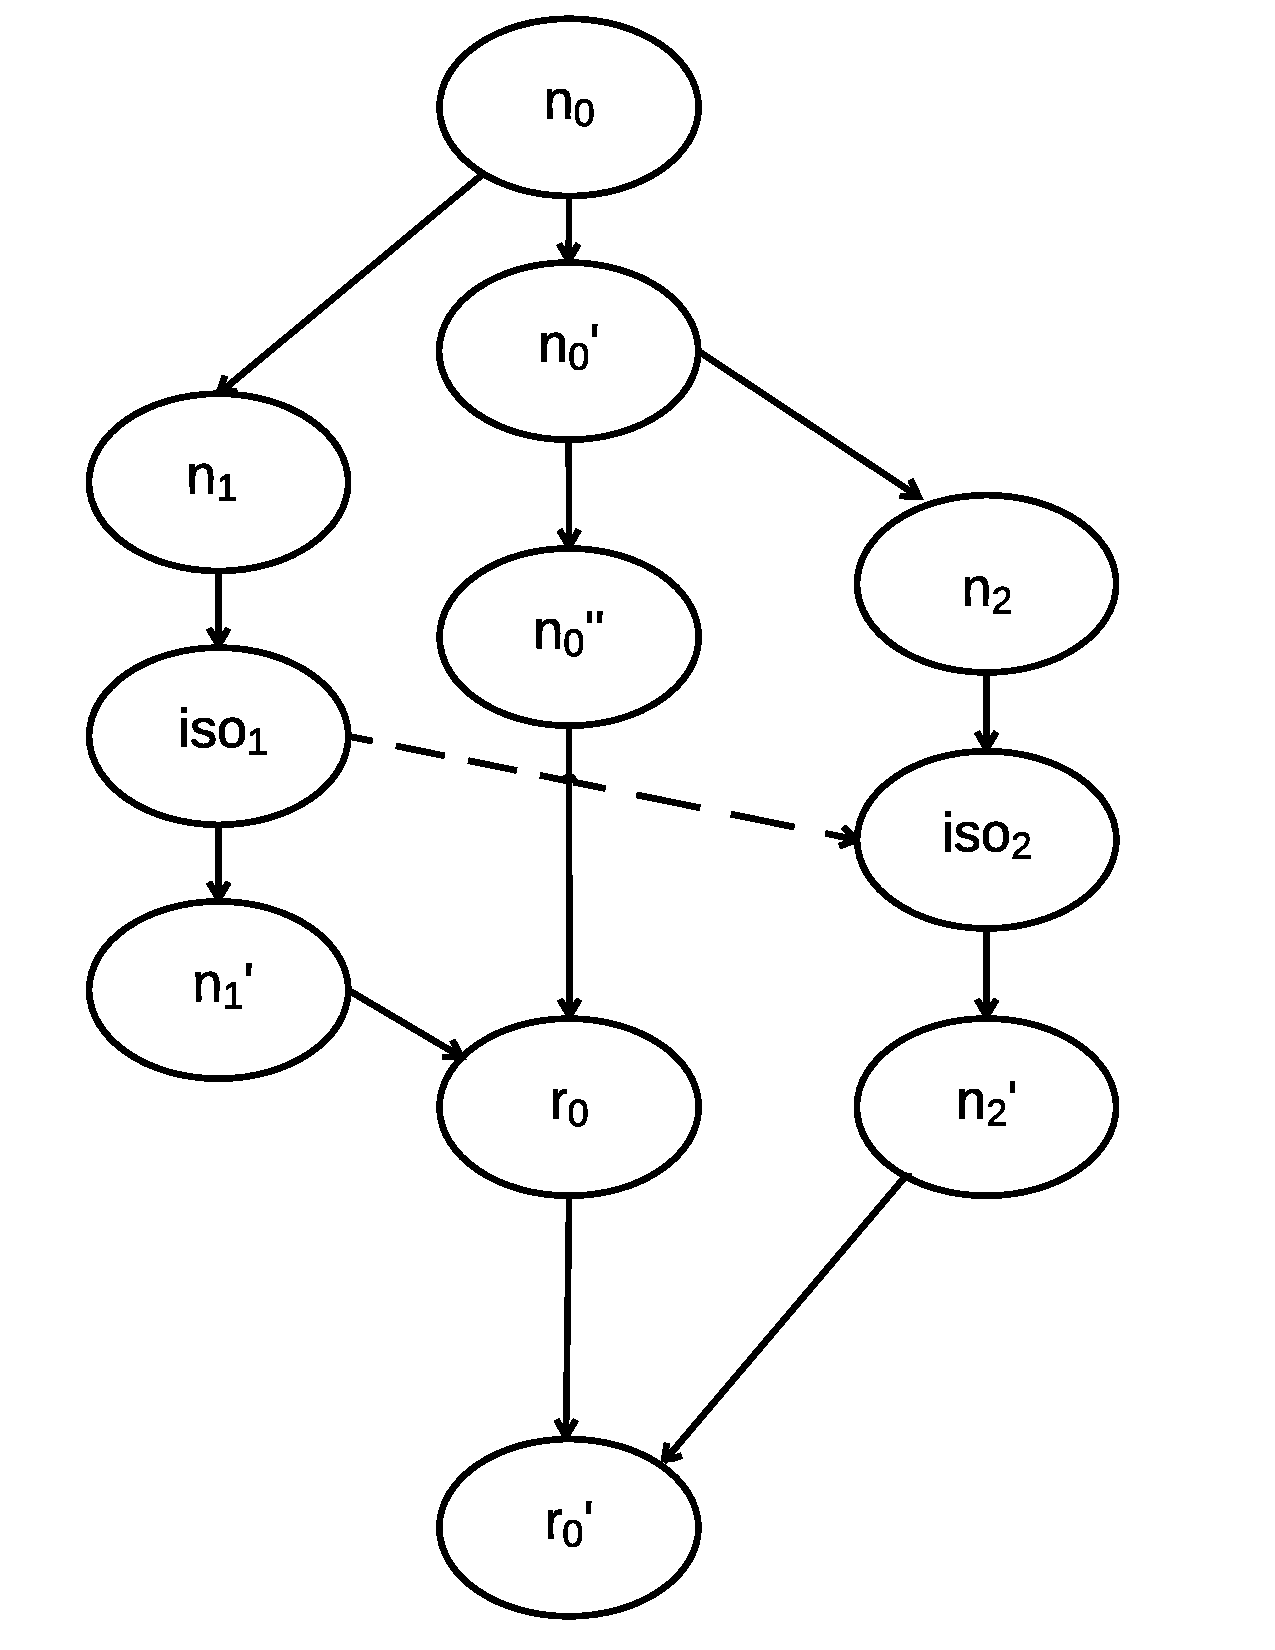
\includegraphics[scale=0.2]{../figs/Fig5-a.pdf}}
  \subfigure[p1 runs before p2.]{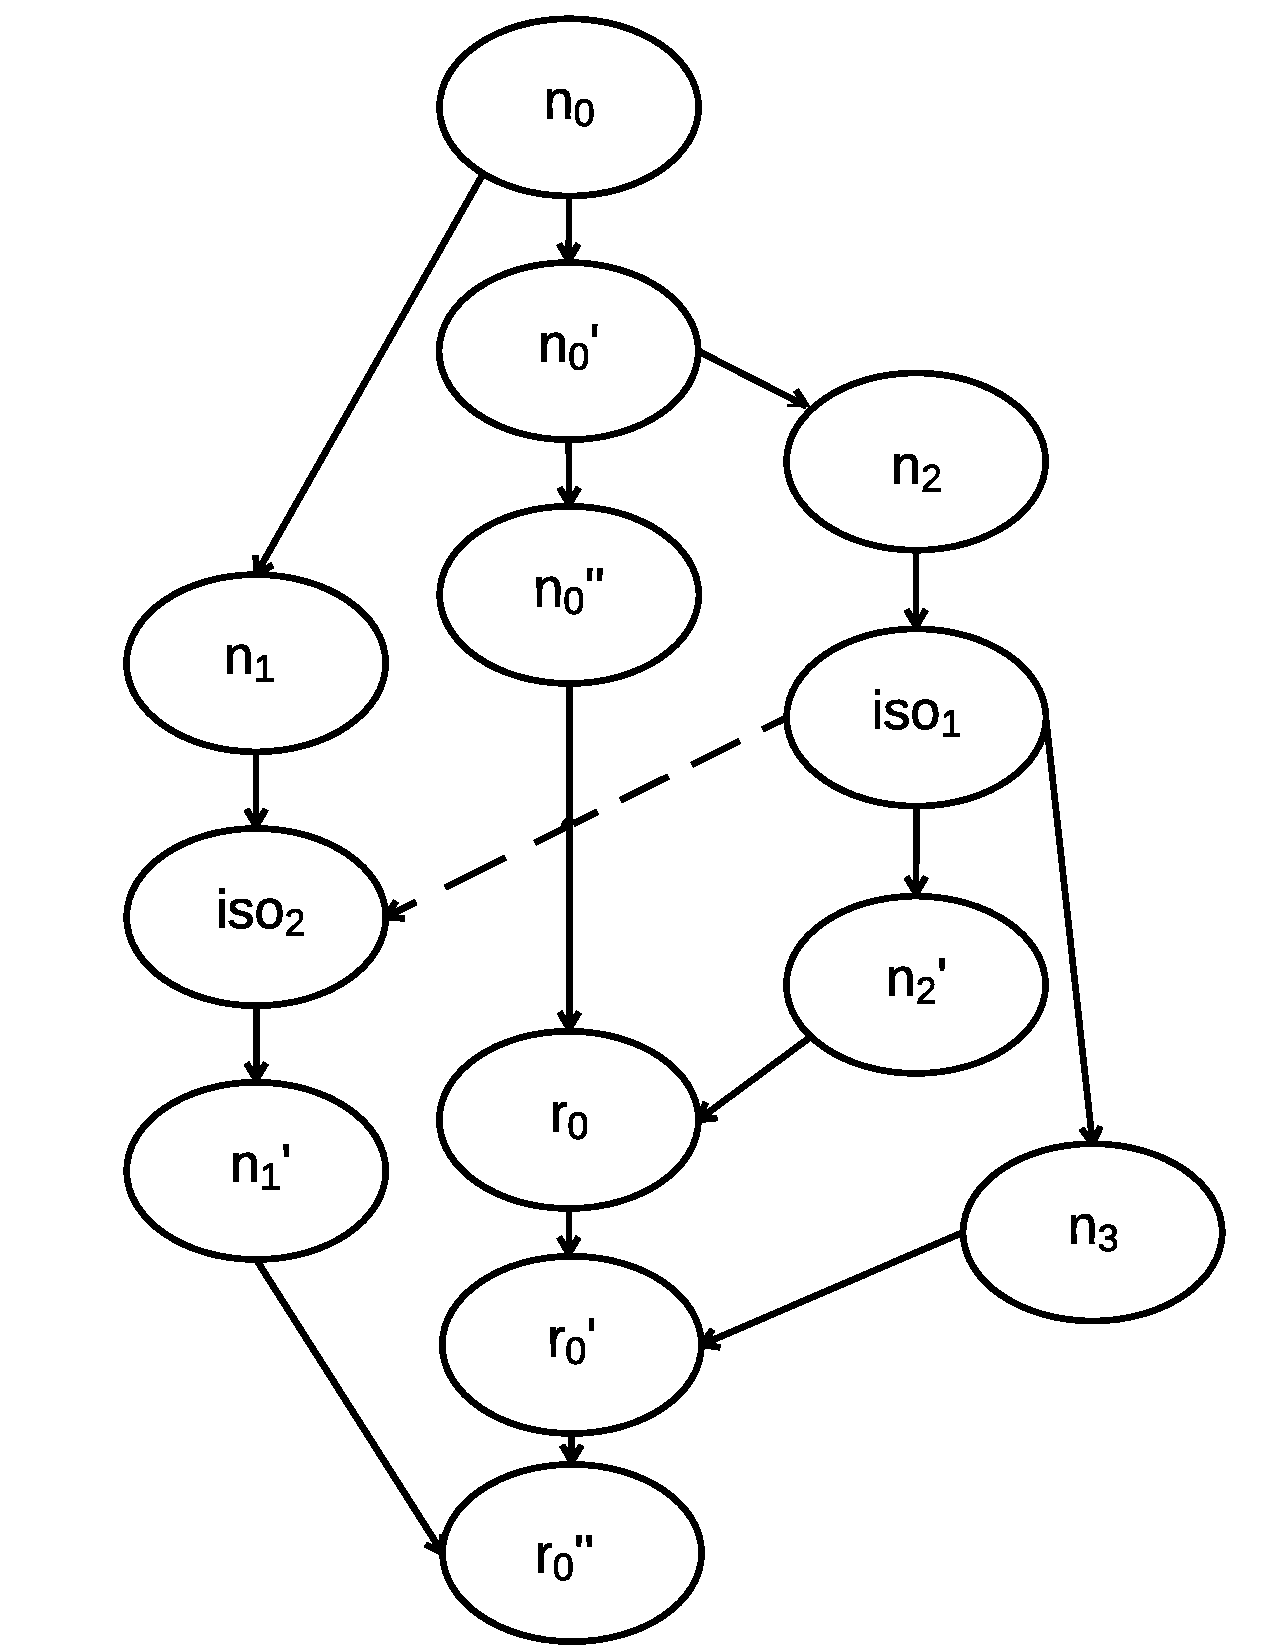
\includegraphics[scale=0.2]{../figs/Fig5-b.pdf}}
  \caption{Two possible computation graphs based on isolated schedules.}
  \vspace{-1em}
   \label{fig:cg-isolated}
\end{figure}

For the example in \figref{fig:hj-isolated}, two different computation graph structures can be formed based on the order of execution of isolated blocks. The computation graphs are shown in \figref{fig:cg-isolated}. The main task spawns two new tasks $t_1$ and $t_2$ both having isolated sections that run in mutual exclusion to each other. All the tasks have read/write access to region variable $r_1$. The isolated blocks are serialized by the runtime and based on the scheduler any task can execute its isolated section first. If the scheduler runs the isolated section of task $t_1$ first, the computation graph in \figref{fig:cg-isolated}(a) is formed. Task $t_1$ changes the values of shared variable $r_1$ to 2. Hence, when task $t_2$ executes its isolated section, the if-condition fails and an additional task is not spawned by $t_2$. If the scheduler runs task $t_2$ first, the computation graph of \figref{fig:cg-isolated}(b) is formed. In this schedule, task $t_2$ executes its isolated section first. Since the value of variable $r_1$ is 0, the if-condition is met and a new task is created by $t_2$.

\begin{theorem}
Algorithm \ref{algo:isolated} finds all unique computation graphs for structured parallel programs with isolated sections making it sound and complete with Algorithm \ref{algo:drd}.
\end{theorem}

\begin{proof}
%Theorem \ref{thm:strcutured-par-progs} 
\thmref{thm:strcutured-par-progs} 
states that Algorithm \ref{algo:drd} is sound and complete for structured parallel programs that do not contain isolated sections. If mutual exclusion is present, Algorithm \ref{algo:drd} does not remain sound since different computation graph structures can be formed for such programs. Algorithm \ref{algo:isolated} helps to enumerate all such computation graph structures. Therefore, the data race detection using Algorithm \ref{algo:drd} becomes sound and complete when it is used along with Algorithm \ref{algo:isolated} for structured parallel programs that have mutual exclusion.
\end{proof}
